\documentclass[12pt,a4paper]{article}
\usepackage[utf8]{inputenc}
\usepackage[spanish,es-tabla]{babel}
\usepackage{geometry}
\usepackage{graphicx}
\usepackage{multirow}
\usepackage{tabularx}
\usepackage{mathptmx}
\usepackage{fancyhdr}
\usepackage{array}
\usepackage[table]{xcolor}
\usepackage{titlesec}
\usepackage{setspace}
\usepackage{microtype}
\usepackage{lastpage}
\usepackage{booktabs}
\usepackage{enumitem}
\usepackage{amsmath}
\usepackage{amsfonts}
\usepackage{amssymb}

\graphicspath{{images/}{../images/}{./}}

\geometry{
    top=4.7cm,
    bottom=2.5cm,
    left=2.5cm,
    right=2.5cm,
    headheight=3.9cm,
    headsep=0.4cm
}

\setstretch{1.15}
\setlength{\parindent}{0pt}
\setlength{\parskip}{0.45em}
\setlength{\tabcolsep}{4pt}

\titleformat{\section}
  {\normalfont\fontsize{12}{14.5}\bfseries}{\thesection.}{0.6em}{\uppercase}
\titlespacing*{\section}
  {0pt}{1.8ex plus 0.4ex minus 0.2ex}{0.6ex plus 0.2ex}

\titleformat{\subsection}
  {\normalfont\fontsize{11.5}{13.5}\bfseries}{\thesubsection.}{0.5em}{}
\titlespacing*{\subsection}
  {0pt}{1.4ex plus 0.3ex minus 0.1ex}{0.4ex plus 0.1ex}

\titleformat{\subsubsection}
  {\normalfont\fontsize{10.5}{12.5}\bfseries\itshape}{\thesubsubsection.}{0.4em}{}
\titlespacing*{\subsubsection}
  {0pt}{1.1ex plus 0.2ex minus 0.1ex}{0.3ex plus 0.1ex}

\newcolumntype{Y}{>{\centering\arraybackslash}X}
\newcolumntype{L}{>{\raggedright\arraybackslash}X}
\newcolumntype{C}{>{\centering\arraybackslash}X}

\definecolor{headerblue}{RGB}{26, 54, 93}
\definecolor{darkblue}{RGB}{43, 108, 176}
\definecolor{lightgraybg}{RGB}{248, 248, 248}
\definecolor{tableheader}{RGB}{232, 238, 246}

\newcommand{\docCodigo}{TI-SIGE-ENT-F3-010}
\newcommand{\docVersion}{1.0}
\newcommand{\docProceso}{DESARROLLO CORE / MIDDLEWARES VALIDATION GATES}
\newcommand{\docElaboracion}{29/09/2026}
\newcommand{\docRevision}{29/09/2026}
\newcommand{\docTitulo}{REGLAS DE NEGOCIO Y VALIDATION GATES EN EXPRESS V5}
\newcommand{\docOrganizacion}{FACULTAD DE INGENIERÍA EN SISTEMAS, ELECTRÓNICA E INDUSTRIAL}
\newcommand{\docSubOrganizacion}{CARRERA DE INGENIERÍA DE SOFTWARE}

\newcommand{\encabezadofrecuente}{%
    \renewcommand{\arraystretch}{1.15}%
    \noindent\makebox[\textwidth][c]{%
    \begin{tabularx}{\textwidth}{|>{\centering\arraybackslash}m{2.8cm}|Y|>{\centering\arraybackslash}m{4.8cm}|}
        \hline
        \multirow{4}{2.8cm}{\centering\raisebox{-1.15cm}{
\includegraphics[width=2.5cm,height=2.0cm,keepaspectratio]{images/logo.png}}}
        & \textbf{\fontsize{9}{11}\selectfont \docOrganizacion} 
        & \textbf{\fontsize{8}{10}\selectfont CÓDIGO:} \fontsize{8}{10}\selectfont \docCodigo \\
        \cline{3-3}
        & \textbf{\fontsize{8.5}{10.5}\selectfont \docSubOrganizacion} 
        & \textbf{\fontsize{8}{10}\selectfont VERSIÓN:} \fontsize{8}{10}\selectfont \docVersion \\
        \cline{2-3}
        & \textbf{\fontsize{8}{10}\selectfont PROCESO:} \fontsize{8}{10}\selectfont \docProceso 
        & \textbf{\fontsize{8}{10}\selectfont ELABORACIÓN:} \fontsize{8}{10}\selectfont \docElaboracion \\
        \cline{2-3}
        & \textbf{\fontsize{8.5}{10.5}\selectfont \docTitulo} 
        & \textbf{\fontsize{8}{10}\selectfont ÚLTIMA REVISIÓN:} \fontsize{8}{10}\selectfont \docRevision \\
        \hline
    \end{tabularx}%
    }%
}

\pagestyle{fancy}
\fancyhf{}
\fancyhead[C]{\encabezadofrecuente}
\fancyfoot[C]{\fontsize{10}{12}\selectfont Página \thepage\ de \pageref{LastPage}}
\renewcommand{\headrulewidth}{0pt}

\begin{document}

\noindent{\fontsize{10.5}{12.5}\selectfont \textbf{Integrantes:} Heidi Villavicencio \quad$\vert$\quad Steeven Toala \quad$\vert$\quad Nixon Hurtado \quad$\vert$\quad Andrea Vásquez}

\vspace{0.25cm}

\section{Título}
\textbf{Denominación del Entregable:} Reglas de Negocio y Validation Gates con Middlewares Express v5 -- Código EDT: 3.10

\section{Introducción}
Aunque la interfaz de usuario proporcione validaciones reactivas, la seguridad y confiabilidad de un sistema institucional exigen que la integridad de las reglas de negocio se aplique rigurosamente en el servidor (Server-Side Enforcement). En esta actividad se desarrolló el paquete de middlewares interceptores en Express v5 (\texttt{validation.middleware.js} y \texttt{documento.validator.js}), implementando los Validation Gates conceptualizados en la Fase 1 como compuertas lógicas inquebrantables que impiden el avance de documentos incompletos, sin evidencias o inconsistentes.

\section{Objetivo}
\subsection{Objetivo General}
Implementar los middlewares de validación estricta y compuertas lógicas (Validation Gates) en Express v5, garantizando el cumplimiento irrestricto de las reglas SGC a nivel de servidor.
\subsection{Objetivos Específicos}
\begin{itemize}[leftmargin=1.5em, itemsep=2pt]
    \item Implementar el validador \texttt{validatePonderacion100} en endpoints de envío.
    \item Construir la compuerta \texttt{gateEvidenciasObligatorias} que bloquea avances sin respaldo en MinIO.
    \item Estructurar respuestas semánticas de error con códigos estandarizados y mensajes claros para la interfaz.
\end{itemize}

\section{Alcance}
\subsection{Límites del Entregable (In-Scope)}
\begin{itemize}[leftmargin=1.5em, itemsep=2pt]
    \item Interceptores de validación para las rutas de envío a revisión y suscripción de firmas.
    \item Códigos de error semánticos: \texttt{ERR\_PONDERACION\_INVALIDA}, \texttt{ERR\_EVIDENCIA\_FALTANTE}.
\end{itemize}
\subsection{Exclusiones (Out-of-Scope)}
\begin{itemize}[leftmargin=1.5em, itemsep=2pt]
    \item Validación de interfaces cliente (cubierto en EDT 3.9).
\end{itemize}

\section{Definiciones}
\begin{itemize}[leftmargin=1.5em, itemsep=2pt]
    \item \textbf{Express Middleware:} Función con acceso al objeto de solicitud (\texttt{req}), al objeto de respuesta (\texttt{res}) y a la siguiente función de middleware (\texttt{next}) en el ciclo solicitud-respuesta.
    \item \textbf{Server-Side Enforcement:} Principio de seguridad donde toda regla crítica se evalúa en el servidor, independientemente de las comprobaciones del navegador.
    \item \textbf{HTTP 422 Unprocessable Entity:} Código de estado que indica que el servidor comprende el tipo de contenido pero no puede procesar las instrucciones contenidas debido a errores semánticos.
\end{itemize}

\section{Responsabilidades}
\begin{itemize}[leftmargin=1.5em, itemsep=2pt]
    \item \textbf{Nixon Hurtado / Steeven Toala (Responsables EDT 3.10):} Desarrollo del pipeline de middlewares de validación en Express v5.
    \item \textbf{Andrea Vásquez (Frontend):} Manejo de respuestas 422 y visualización de errores semánticos en el cliente.
    \item \textbf{Ing. Paulo Torres (Docente Evaluador):} Aprobación del rigor de las compuertas lógicas en el servidor.
\end{itemize}

\section{Normativa Legal y Técnica}
\begin{itemize}[leftmargin=1.5em, itemsep=2pt]
    \item \textbf{Express v5 Middleware Architecture.}
    \item \textbf{RFC 4918 (HTTP Status Code 422 Unprocessable Entity).}
\end{itemize}

\section{Método, Políticas y Contenidos}
Se utilizó encadenamiento de middlewares en Express. En la Figura \ref{fig:f3_10_gates} se presenta el árbol de decisión algorítmico ejecutado por las compuertas en el backend.

\begin{figure}[htbp]
    \centering
    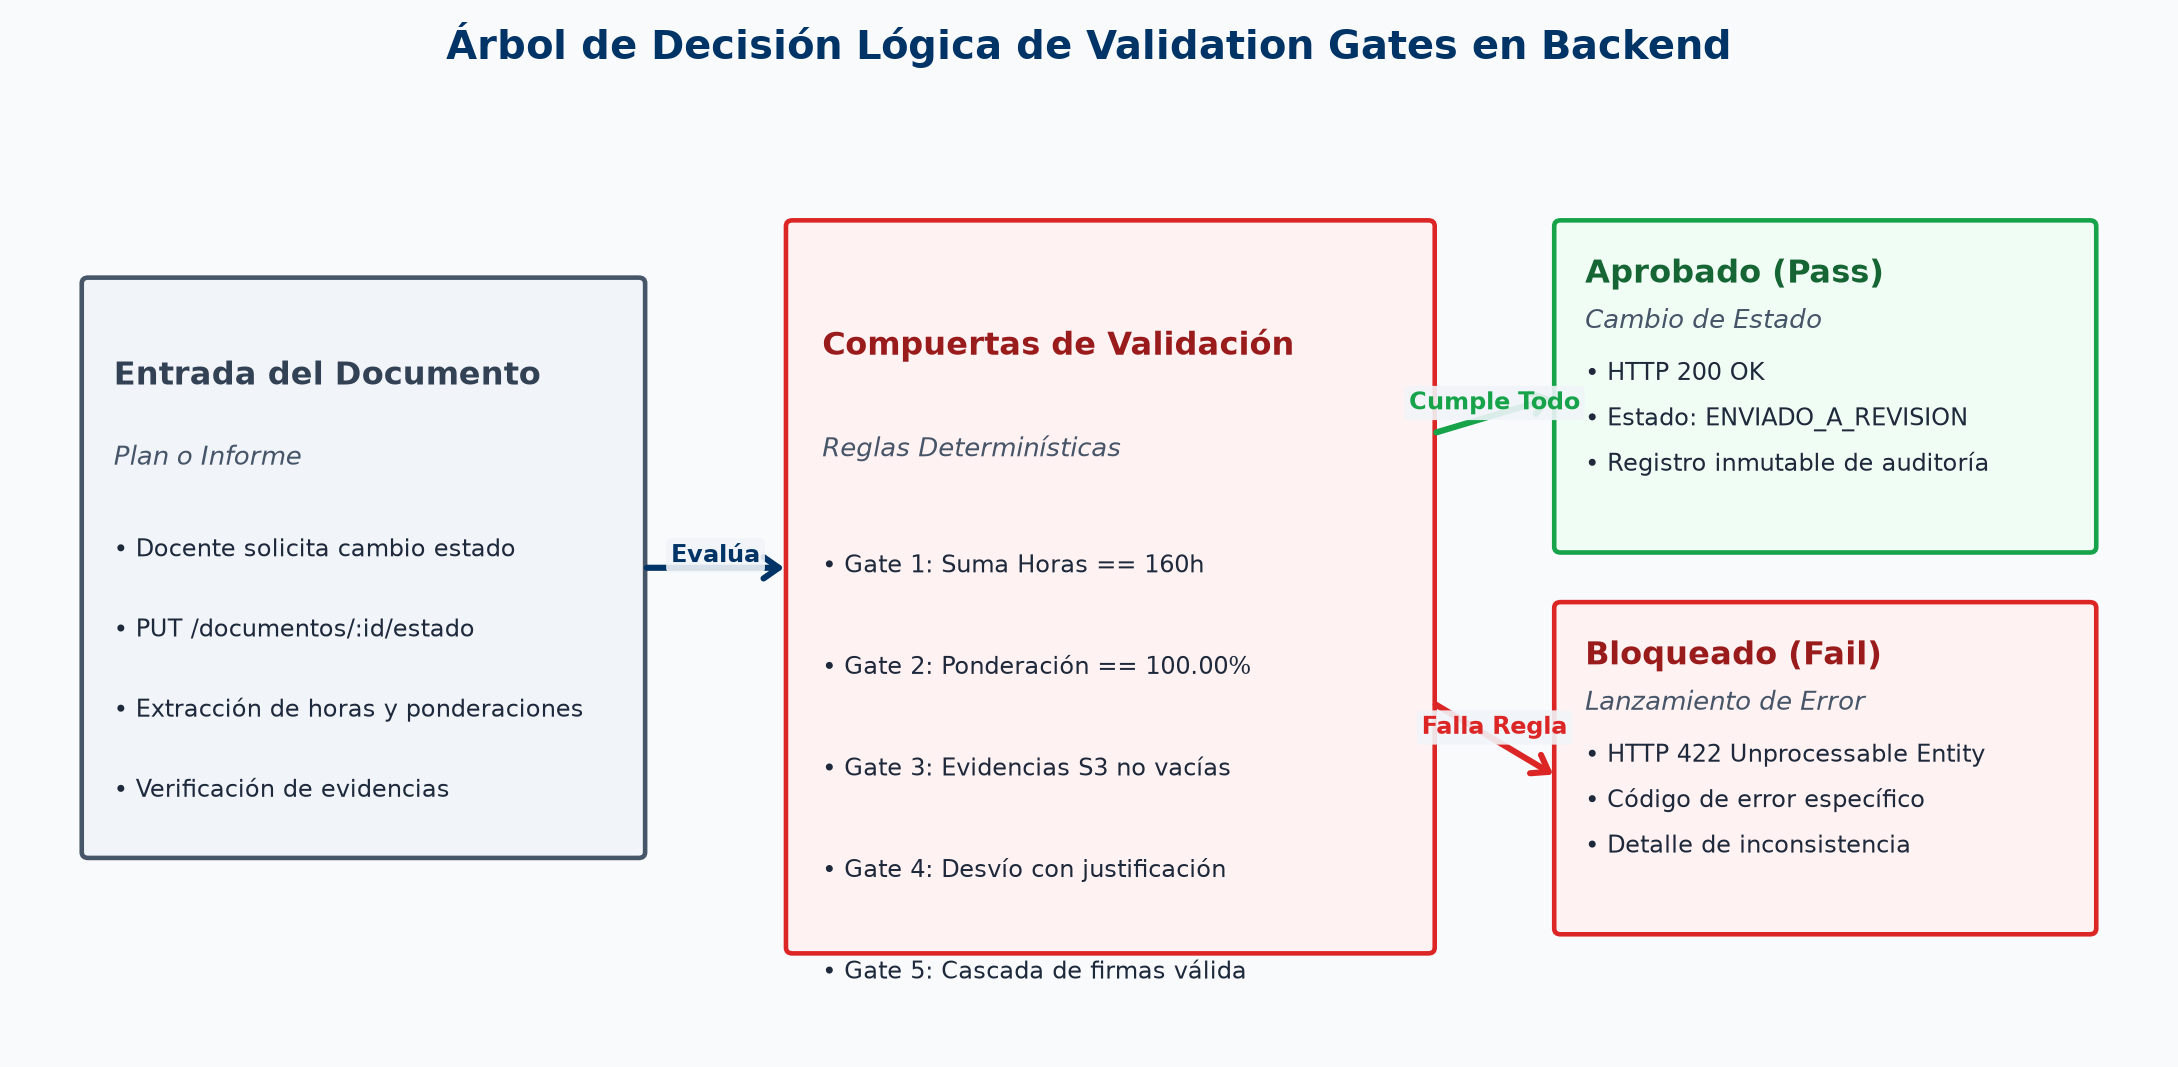
\includegraphics[width=0.88\textwidth,height=5.5cm,keepaspectratio]{images/f3_09_decision_validation_gates.png}
    \caption{Árbol de Decisión Algorítmico y Middlewares de Validation Gates en Express v5.}
    \label{fig:f3_10_gates}
\end{figure}

\section{Descripción de actividades}
\subsection{Matriz de Compuertas Lógicas y Errores Semánticos}
\begin{table}[htbp]
\centering
\small
\renewcommand{\arraystretch}{1.2}
\begin{tabularx}{\textwidth}{|>{\bfseries}m{2.5cm}|X|c|X|}
\hline
\rowcolor{tableheader}
\textbf{Compuerta} & \textbf{Condición de Evaluación en Backend} & \textbf{HTTP Status} & \textbf{Código de Error Semántico} \\
\hline
Gate 1: Ponderación & $|(\sum P_i) - 100.00| > 0.01$ en la matriz de actividades. & 422 & \texttt{ERR\_PONDERACION\_INVALIDA} \\
\hline
Gate 2: Evidencias & Actividad con $A_i > 0\%$ sin evidencia registrada en MinIO. & 422 & \texttt{ERR\_EVIDENCIA\_FALTANTE} \\
\hline
Gate 3: Fechas & Fechas de actividad fuera del rango del período lectivo. & 400 & \texttt{ERR\_FECHA\_FUERA\_PERIODO} \\
\hline
Gate 4: Extemporáneo & Documento enviado fuera de fecha límite sin token de desbloqueo. & 403 & \texttt{ERR\_ENVIO\_EXTEMPORANEO} \\
\hline
Gate 5: Cascada & Intento de firma de nivel 2 sin firma de nivel 1 validada. & 409 & \texttt{ERR\_CASCADA\_FIRMADA\_PREVIA} \\
\hline
\end{tabularx}
\caption{Especificación de Validation Gates y Respuestas Semánticas.}
\label{tab:gates_backend}
\end{table}

\subsection{Protección Contra Evasión de Validaciones}
Cualquier petición manual hacia los endpoints de envío que intente eludir el frontend es interceptada inmediatamente por el pipeline de Express, devolviendo una respuesta JSON explicativa que protege la integridad de la base de datos institucional.

\section{Firmas de Responsabilidad}

\noindent
\renewcommand{\arraystretch}{1.2}
\begin{tabularx}{\textwidth}{|>{\raggedright\arraybackslash}m{2.9cm}|>{\raggedright\arraybackslash}X|>{\centering\arraybackslash}m{4.6cm}|>{\centering\arraybackslash}m{2.3cm}|}
    \hline
    \rowcolor{tableheader}
    \textbf{ACCIÓN} & \textbf{NOMBRE Y CARGO} & \textbf{FIRMA} & \textbf{FECHA} \\
    \hline
    \textbf{Elaborado por:} & Heidi Villavicencio\newline Analista de Calidad / UI-UX & \parbox[c]{4.4cm}{\centering\vspace{4pt}
\includegraphics[height=1.5cm,width=4.0cm,keepaspectratio]{images/firma_heidi.png}\vspace{4pt}} & 29/09/2026 \\
    \hline
    \textbf{Revisado por:} & Steeven Toala\newline Líder de Proyecto / Arquitecto & \parbox[c]{4.4cm}{\centering\vspace{4pt}
\includegraphics[height=1.5cm,width=4.0cm,keepaspectratio]{images/firma_steveen.png}\vspace{4pt}} & 29/09/2026 \\
    \hline
    \textbf{Aprobado por:} & Ing. Paulo Torres, Mg.\newline Docente Evaluador -- Gestión Proyectos & \parbox[c]{4.4cm}{\centering\vspace{8pt}\textbf{\textcolor{gray!80}{\scriptsize [ PENDIENTE DE APROBACIÓN ]}}\vspace{8pt}} & \textbf{\textcolor{gray!90}{Pendiente}} \\
    \hline
\end{tabularx}

\vspace{0.4cm}

\section{Control de Cambios}

\noindent
\renewcommand{\arraystretch}{1.2}
\begin{tabularx}{\textwidth}{|>{\hsize=0.45\hsize\centering\arraybackslash}X|>{\hsize=1.55\hsize\raggedright\arraybackslash}X|>{\hsize=1.2\hsize\raggedright\arraybackslash}X|>{\hsize=0.8\hsize\centering\arraybackslash}X|}
    \hline
    \rowcolor{tableheader}
    \textbf{Versión} & \textbf{Descripción del cambio} & \textbf{Responsable del cambio} & \textbf{Fecha de aprobación} \\
    \hline
    1.0 & Emisión inicial del entregable según EDT del Tablero Trello & Equipo de Proyecto SIGE & 29/09/2026 \\
    \hline
\end{tabularx}

\vspace{0.4cm}

\section{Anexos}
\begin{itemize}[leftmargin=1.5em]
\item \textbf{Anexo 1:} Registros de Bloqueo Exitoso en Pruebas de Carga Malformada.
\end{itemize}

\end{document}
